\chapter{الدوال غير المستمرة}

\section{نقاط عدم الاستمرارية}

\begin{definition}[( نقاط عدم الاسترمرارية ) \cite{mathanalysis}]
	نقول  ان $x=c$ هي نقطة عدم استمرارية اذا كانت $f$ غير مستمرة عند $c$
\end{definition}

\noindent
\textbf{ملاحظة}\\
في هذه الحالة واحدة من الحالات الاتية متحقق
\begin{enumerate}
	\item اما $f(c^+)$ او $f(c^-)$ غير موجودة.
	\item كلا $f(c^+)$ و $f(c^-)$ موجود ولكن لهما قيم مختلفة اي ان $f(c^+) \neq f(c^-)$
\item كلا $f(c^+)$ و $f(c^-)$ موجودة ولكن $f(c^+) = f(c^-) \neq f(c)$.
\end{enumerate}
\vspace{5pt}
\noindent
\textbf{امثلة على الحالات الثلاثة}
\begin{enumerate}
	\item الدالة $f(x) = \sqrt{x}$ معرفة على الفترة $[0, \infty]$ اي ان $f(0-)$ غير موجودة وبالتالي $x=0$ هي نقطة عدم استمرارية
	\item الدالة
	\[
	f(x) =
	\begin{cases}
		x^2 + 1 & x\leq 1 \\
		x & x>1
	\end{cases}
	\]
	غير مستمرة عند $x=1$ لان 
	$f(1^+) = 1 \neq 2 = f(1^-)$
	\begin{figure}[H]
		\centering
		\begin{tikzpicture}
			\begin{axis}[
				axis lines = middle,
				xlabel = \( x \),
				ylabel = \( f(x) \),
				domain = -2:3,
				samples = 100,
				]
				% Plot for x <= 1
				\addplot[blue, thick, domain=-2:1] {x^2 + 1};
				% Plot for x > 1
				\addplot[red, thick, domain=1:3] {x};
			\end{axis}
		\end{tikzpicture}
		\caption{\en{Plot of \( f(x) \)}}
	\end{figure}
	
	\item الدالة
	\[
	f(x) = 
	\begin{cases}
		1 & x=0 \\
		x+2 & x>0\\
		x^2+2& x<0
	\end{cases}
	\]
	غير مستمرة عند $x=-1$ لان $f(0) = 1$ ولكن $f(0^+) = 2=f(0^-)$
	\begin{figure}[H]
		\centering
		\begin{tikzpicture}
			\begin{axis}[
				axis lines = middle,
				xlabel = \( x \),
				ylabel = \( f(x) \),
				domain = -3:3,
				samples = 100,
				restrict y to domain=-1:10, % to prevent overflow in plot at x = 0
				]
				% Plot for x < 0 (x^2 + 2)
				\addplot[blue, thick, domain=-3:0] {x^2 + 2};
				% Plot for x > 0 (x + 2)
				\addplot[red, thick, domain=0.01:3] {x + 2}; % Starts slightly after 0 to avoid overlap
				% Mark the point at x = 0
				\addplot[mark=*, only marks, black] coordinates {(0, 1)};
			\end{axis}
		\end{tikzpicture}
				\caption{\en{Plot of \( f(x) \)}}
	\end{figure}
\end{enumerate}

\begin{definition}[( عدم الاستمرارية القابلة للحذف ) \cite{mathanalysis}]
	لتكن $f$ دالة معرفة على الفترة $[a, b]$ و $c\in [a, b]$ فإن $c$ تكون نقطة عدم استمرارية قابلة للحذف اذا كان $f(c^+) = f(c^-) \neq f(c)$. ويتم حذف عدم الاستمرارية بإعادة تعريف الدالة $f$ عند $c$ حيث يكون  $f(c^+) = f(c^-) = f(c)$.
\end{definition}

\begin{definition}[( عدم الاستمرارية غير القابلة للحذف ) \cite{mathanalysis}]
	لتكن $f$ دالة معرفة على الفترة $[a, b]$ فإن $c$ تكون نقطة عدم استمرارية غير قابلة للحذف اذا كانت $f(c^+)$ غير موجودة او $f(c^-)$ غير موجودة او $f(c^+) \neq f(c^-)$
\end{definition}

\begin{definition}[( عدم الاستمرارية القفزية ) \cite{mathanalysis}]
	لتكن $f$ دالة معرفة على الفترة المغلقة $[a, b]$ اذا كانت كلا $f(c^+)$ و $f(c^-)$ موجودة على نقطة داخلية مثل $c$ فإن:
	\begin{enumerate}
		\item $f(c) - f(c^-)$ تسمى بالقفزة من اليسار 
		\item  $f(c^+) - f(c)$ تسمى بالقفزة من اليمين
		\item $f(c^+) - f(c^-)$ تسمى بالقفزة
	\end{enumerate}
	اذا كانت واحدة من القيم الثلاثة اعلاه لاتساوي صفراً. فإن $c$ تسمى نقطة عدم استمرارية قفزية\\ \en{Jump Discontinuty}
\end{definition}

\noindent
\textbf{ملاحظة}\\
بالنسبة لنهايتي الفترة $a, b$ فقط القفزة من جهو واحدة  تأخذ بعين الاعتبار. بالنسبة الى $a$ ناخذ\\ $f(a^+) - f(a)$ وبالنسبة الى $b$ ناخذ $f(b) - f(b^-)$


\begin{definition}[( عدم الاستمرارية الاساسية ) \cite{mathanalysis}]
 	تكون الدالة $f(x)$ تمتلك عدم استمرارية اساسية \LR{essential discontinuty}
عند $x=c$ اذا كانت الغاية 
$\lim\limits_{x\to c} f(x)$ غير موجودة. وعلى الاقل واحدة من الغايات اليمينية او اليسارية ايضاً غير موجودة (ربما كليهما).
\end{definition}

\noindent
الآن نلخص انواع عدم الاستمرارية
\begin{enumerate}
	\item عدم الاستمرارية قابلة للحذف \LR{removable discontinuty}.
\item عدم الاستمرارية غير قابلة للحذف \LR{non-romvable discontinuty}.
\item عدم الاستمرارية القفزية \LR{jump discontinuty}.
\item عدم الاستمرارية الاساسية \LR{essential discontinuty}.
\end{enumerate}
الآن نأخذ بعض الامثلة لنغطي على جميع الانواع.
\newpage
\begin{example}
	الدالة $f(x) = x/|x|$ تمتلك عدم استمرارية قفزية عند $x=0$ لان 
	\[
	f(0^+) = 1,\quad f(0^-) = -1
	\]
	
	\begin{figure}[H]
		\centering
		\begin{tikzpicture}
		\begin{axis}[
			axis lines = middle,
			xlabel = \( x \),
			ylabel = \( f(x) \),
			domain = -3:3,
			samples = 100,
			ymin = -2, ymax = 2,
			restrict y to domain=-2:2, % Restrict y values to avoid infinity at x = 0
			]
			% Plot for x > 0 (f(x) = 1)
			\addplot[blue, thick, domain=0.01:3] {1};
			% Plot for x < 0 (f(x) = -1)
			\addplot[red, thick, domain=-3:-0.01] {-1};
			% Mark the undefined point at x = 0
			\addplot[mark=*, only marks, black] coordinates {(0, 0)};
		\end{axis}
		\end{tikzpicture}
		\caption{\en{Plot of \( f(x) = x/|x| \)}}
	\end{figure}
\end{example}

\begin{example}
	الدالة
	\[
	f(x) =
	\begin{cases}
		1 & x\neq0 \\
		0 & x=0
	\end{cases}
	\]
	تمتلك عدم استمرارية قابلة للحذف عند $x=0$ لان 
	\begin{align*}
		& f(0) = 0\\
		& f(0^+) = f(0^-) = 1
	\end{align*}
\end{example}

\begin{example}
	الدالة
	\[
	f(x) =
	\begin{cases}
		\dfrac{1}{x}& x\neq0 \\
		A & x=0
	\end{cases}
	\]
	تمتلك عدم استمرارية غير قابلة للحذف عند $x=0$ لان $f(c^-), f(c^+)$ غير موجودة
	
	\begin{figure}[H]
		\centering
		\begin{tikzpicture}
			\begin{axis}[
				axis lines = middle,
				xlabel = \( x \),
				ylabel = \( f(x) \),
				domain = -2.5:2.5,
				samples = 200,
				restrict y to domain=-5:5, % Limit y to make the oscillations visible
				]
				% Plot for x != 0 (sin(1/x))
				\addplot[blue, thick, domain=-1.5:-0.01] {1/x};
				\addplot[blue, thick, domain=0.01:1.5] {1/x};
				% Mark the point at x = 0 where f(x) = 1
				\addplot[mark=*, only marks, thick] coordinates {(0, 1)};
			\end{axis}
		\end{tikzpicture}
		\caption{\en{Plot of \( f(x) = 1/x \) for \( x \neq 0 \)}}
	\end{figure}
\end{example}

\begin{example}
	الدالة
	\[
	f(x) =
	\begin{cases}
	\sin\dfrac{1}{x}& x\neq0 \\
		A & x=0
	\end{cases}
	\]
	تمتلك عدم استمرارية غير قابلة للحذف عند $x=0$ لان $f(0^-), f(0^+)$ غير موجودة (لان كلما كان قيمة $x$ تقترب من الصفر سواء من اليمين او من اليسار فإن قيمة الدالة $f$ تتناوب بين $-1$ و 1 وكما موضح في الشكل 2 - 5)
	\begin{figure}[H]
		\centering
		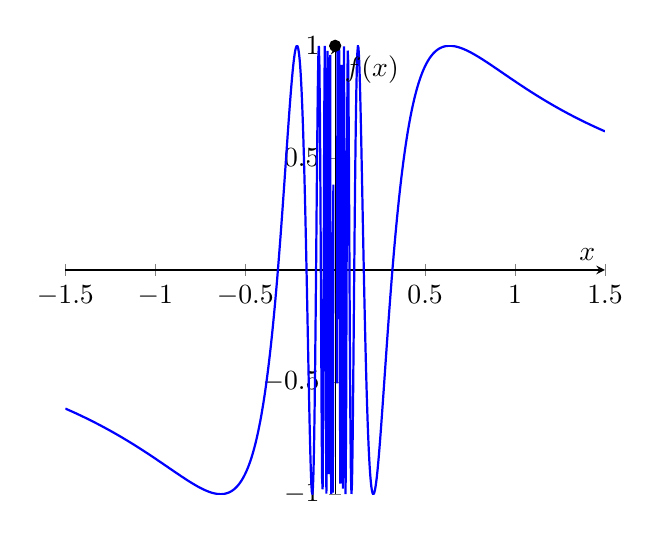
\begin{tikzpicture}
			\begin{axis}[
				axis lines = middle,
				xlabel = \( x \),
				ylabel = \( f(x) \),
				domain = -1.5:1.5,
				samples = 500,
				restrict y to domain=-2:2, % Limit y to make the oscillations visible
				]
				% Plot for x != 0 (sin(1/x))
				\addplot[blue, thick, domain=-1.5:-0.01] {sin(deg(1/x))};
				\addplot[blue, thick, domain=0.01:1.5] {sin(deg(1/x))};
				% Mark the point at x = 0 where f(x) = 1
				\addplot[mark=*, only marks, black] coordinates {(0, 1)};
			\end{axis}
		\end{tikzpicture}
		\caption{\en{Plot of \( f(x) = \sin(1/x) \) for \( x \neq 0 \)}}
	\end{figure}
\end{example}
\newpage
\begin{example}
	الدالة
	\[
	f(x) =
	\begin{cases}
		x\sin \dfrac{1}{x} & x\neq0 \\
		1 & x=0
	\end{cases}
	\]
	تمتلك عدم استمرارية قابلة للحذف لان
	 $f(0+) = f(0-) = 0$
	 و $f(0) = 1$ 
	 	\begin{figure}[H]
	 	\centering
	 	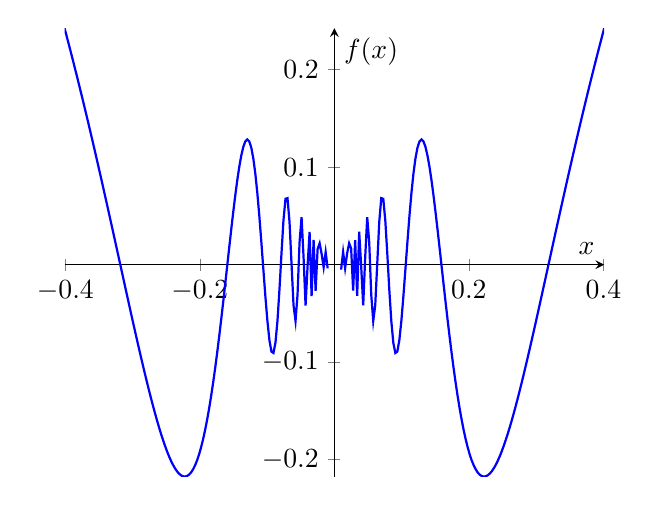
\begin{tikzpicture}
	 		\begin{axis}[
	 			axis lines = middle,
	 			xlabel = \( x \),
	 			ylabel = \( f(x) \),
	 			domain = -1.5:1.5,
	 			samples = 500,
	 			restrict y to domain=-2:0.25, % Limit y to make the oscillations visible
	 			]
	 			% Plot for x != 0 (sin(1/x))
	 			\addplot[blue, thick, domain=-1.5:-0.01] {x*sin(deg(1/x))};
	 			\addplot[blue, thick, domain=0.01:1.5] {x*sin(deg(1/x))};
	 			% Mark the point at x = 0 where f(x) = 1
	 			\addplot[mark=*, only marks, black] coordinates {(0, 1)};
	 		\end{axis}
	 	\end{tikzpicture}
	 	\caption{\en{Plot of \( f(x) =x \sin(1/x) \) for \( x \neq 0 \)}}
	 \end{figure}
\end{example}

\begin{example}
	الدالة $f(x) = \exp\left(\dfrac{1}{x}\right)$ تمتلك عدم استمرارية اساسية عند $x=0$ لأن الغايات
	\[
	\lim\limits_{x\to 0} \exp\left(\frac{1}{x}\right), \quad 	\lim\limits_{x\to 0^+} \exp\left(\frac{1}{x}\right), 
	\]
	غير موجودة ولكن 
	\[
		\lim\limits_{x\to 0^-} \exp\left(\frac{1}{x}\right) = 0
	\]
\end{example}

\newpage

\begin{example}
اوجد نقاط عدم الاستمرارية للدالة وصنفها
	\[
	f(x) =
	\begin{cases}
		\dfrac{x^2 - 4}{x -2} & x \neq 2 \\
		1 & x =2
	\end{cases}
	\]
\end{example}
\begin{solution}
 نلاحظ
	\[
	\lim\limits_{x\to 2} f(x) = \lim\limits_{x\to 2} \frac{(x-2)(x+2)}{x-2} = \lim\limits_{x\to 2} x+2 = 4
	\]
	ولكن $f(2) = 1$ اذن $x=2$ نقطة عدم استمرارية قابلة للحذف. وذلك بأعادة تعريف الدالة عند $x=2$ لتكون $f(2) = 4$.
	\end{solution}
	\begin{example}
		اوجد نقاط عدم الاستمرارية وصنفها
		\[
		f(x) = 
		\begin{cases}
			\dfrac{x^2 - 4x +3}{2x-2} & x > 1 \\
			3 & x=1\\
			\dfrac{x^2 - 1}{x-1} & x<1
		\end{cases}
		\]
	\end{example}
	\begin{solution}
		نوجد غاية اليمين عند $x=1$ 
		\[
		\lim\limits_{x\to 1^+} f(x) = \lim\limits_{x\to 1^+} \frac{(x-1)(x-3)}{2(x-1)} = \lim\limits_{x\to 1^+} \frac{x-3}{2} = -1
		\]
		بينما غاية اليسار
		\[
		\lim\limits_{x\to 1^-} f(x) = \lim\limits_{x\to 1^-} \frac{(x-1)(x+1)}{x-1} =\lim\limits_{x\to 1^-} x+1 =2
		\]
		ولكن $f(1)=3$. اذن $x=1$ نقطة عدم استمرارية غير قابلة للحذف لأنه لا يمكن اعادة تعريف الدالة عند $x=1$ لتكون الدالة مستمرة عند تلك النقطة وذلك لأن غاية اليمين لا تساوي غاية اليسار.
	\end{solution}

\newpage
\section[المشتقات عند الدوال غير المستمرة]{المشتقات عند الدوال غير المستمرة \cite{mathanalysis}}
لدراسة الدوال غير المستمرة في الاشتقاق. نقدم مفهوم المشتقة من اتجاه واحد والمشتقة اللا نهائية.
\begin{definition}[( المشتقة من اتجاه واحد )]
	لتكن $f$ دالة معرفة على الفترة المغلقة $[a, b]$ نقول ان $f$ تمتلك مشتقة يمينية عند $c$ اذا كانت الغاية 
	\[
	\lim\limits_{x\to c^+} \frac{f(x) - f(c)}{x-c}
	\]
	موجودة كقيمة نهائية او ان الغاية هي $+\infty$ او $-\infty$ و نرمز لها بالرمز $f_+'(x)$. المشتقة اليسارية تعرف بنفس الاسلوب
	\[
f_-'(c):=	\lim\limits_{x\to c^-} \frac{f(x) - f(c)}{x-c}
	\]
\end{definition}

\begin{example}
	لتكن الدالة $f(x) = |x|$، رأينا في المثال 1 - 3 - 1 ان الدالة لا تمتلك مشتقة عند  $x=0$ ولكن
	\[
f_+'(0) = \lim\limits_{x\to0^+} \frac{|x|}{x} = \lim\limits_{x\to0^+} \frac{x}{x} =1
\]
\[
f_-'(0) = \lim\limits_{x\to0^-} \frac{|x|}{x} = \lim\limits_{x\to0^-} \frac{-x}{x}=- 1
\]

\begin{figure}[H]
	\centering
	\begin{tikzpicture}
		\begin{axis}[
			axis lines = middle,
			xlabel = $x$,
			ylabel = {$f(x)$},
			xmin = -5, xmax = 5,
			ymin = 0, ymax = 5,
			samples = 100
			]
			\addplot[domain=-5:5,blue,thick] {abs(x)};
		\end{axis}
	\end{tikzpicture}
	\caption{$f(x) = |x|$}
\end{figure}
\newpage
\end{example}

\begin{example}
	لتكن 
\[
f(x)=
\begin{cases}
	\dfrac{1}{2}x^2 + 1 & x\leq 2 \\
	x+2 & x>2
\end{cases}
\]	
الدالة غير مستمرة عند $x=2$ لأن 
\[
f(2^+) = 4 \neq 2 = f(2^-)
\]
ولكن 
\begin{align*}
	f_+'(2) &= \lim\limits_{x\to 2^+} \frac{f(x) - f(2)}{x-2} \\
	&= \lim\limits_{x\to 2^+} \frac{x+2-3}{x-2} \\
	&= \lim\limits_{x\to2^+} \frac{x-1}{x-2} = -\infty
\end{align*}
و
\begin{align*}
	f_-'(2) &= \lim\limits_{x\to 2^-} \frac{\dfrac{1}{2} x^2 +1 -3}{x-2}\\
	&= \lim\limits_{x\to 2^-} \frac{\dfrac{1}{2}(x^2-4)}{x-2} \\
	&= \lim\limits_{x\to 2^-} \frac{\dfrac{1}{2}(x-2)(x+2)}{x-2}\\
	&= \lim\limits_{x\to 2^-} \frac{1}{2}(x+2)\\
	&= 2
\end{align*}
\begin{figure}[H]
		\centering
		\begin{tikzpicture}
			\begin{axis}[
				axis lines = middle,
				xlabel = $x$,
				ylabel = {$f(x)$},
				xmin = -5, xmax = 5,
				ymin = -2, ymax = 10,
				samples = 100
				]
				\addplot[domain=-5:2,blue,thick] {0.5*x^2 + 1};
				\addplot[domain=2:5,red,thick] {x + 2};
			\end{axis}
		\end{tikzpicture}
		\caption{\en{Plot of \(f(x)\)}}
\end{figure}
\end{example}

\section[الاستمرارية بالأجزاء]{الاستمرارية بالاجزاء \cite{ode1}}

\begin{definition}[( الاستمرارية بالأجزاء )]
	نقول ان الدالة $f(x)$ مستمرة بالاجزاء على الفترة المغلقة $[a, b]$ اذا كانت مستمرة عند عدد منتهِ من نقاط عدم الاستمرارية القفزية
\end{definition}

\begin{example}
	الدالة 
	\[
	f(x) =
	\begin{cases}
		x^3  & 0\leq x\leq 1 \\
		1-x & 1\leq x \leq 2\\
		1 & 2\leq x \leq 3
	\end{cases}
	\]
\end{example}

\begin{note}
	ليس مطلوب ان تكون الدالة $f(x)$ معرفة عند نقاط عدم الاستمرارية القفزية. لنفر	ض ان $a_1, \dots, a_n$ مواقع عد الاستمرارية القفزية للدالة $f$ في الفترة $[a, b]$ ونفرض ان $a_i < a_{i+1}$ لكل $i$، على الفترة $(a_i, a_{i+1})$ يمكننا جعل $f(x)$ دالة مستمرة على الفترة المغلقة $[a_i, a_{i+1}]$ من خلال تعريف
	\[
	f(a_i) = \lim\limits_{x\to a_i^+}f(x), \quad f(a_{i+1}) = \lim\limits_{x\to a_{i+1}^-} f(x)
	\]
	ولأن الدالة المستمرة على الفترة المغلقة تكون مقيدة لدينا المبرهنة التالية
\end{note}

\begin{theorem}
	اذا كانت $f(x)$ دالة مستمرة بالاجزاء على الفترة $[a, b]$ فإن $f(x)$ تكون مقيدة.
\end{theorem}

\section[تكامل الدوال المستمرة بالاجزاء]{تكامل الدوال المستمرة بالاجزاء \cite{ode2}}

\begin{definition}
	اذا كانت $f(x)$ مستمرة بالاجزاء على الفترة $[a , b]$ ونقاط عدم الاستمرارية عند \\$a_1<a_2<\cdots<a_k$، لتكن $a=a_0, b=a_{k+1}$. كما لاحظنا فإننا من الممكن جعل الدالة $f$ مستمرة على $[a_i, a_{i+1}]$ وبالتالي من الممكن تعريف التكامل المحدد للدالة $f$ على الفترة $[a, b]$ كما يلي
	\[
	\int_{a}^{b} f(x) \, dx = \int_{a_0}^{a_1} f(x)\, dx + \int_{a_1}^{a_2} f(x) \, dx + \cdots + \int_{a_k}^{a_{k+1}} f(x) \, dx
	\]
\end{definition}

\begin{example}
	نجد التكامل للدالة $f(x)$ المعرفة بالشكل
	\[
	f(x) = 
	\begin{cases}
		1 & 0\leq x< 1 \\
		0 & 1\leq x < \infty
	\end{cases}
	\]
	على الفترة $[0, t]$ حيث $t\in [0,\infty)$. لدينا احتمالان هنا:\\
	1. اذا كان $t\in [0,1)$ فإن 
	\[
	\int_{0}^{t} f(x) \, dx = \int_{0}^{t} 1 \, dx = t
	\]
	2. اذا كان $t\in [1, \infty)$ فإن 
	\begin{align*}
		\int_{0}^{t}f(x) \, dx &=\int_{0}^{1}f(x) \, dx + \int_{1}^{t} f(x) \, dx\\
		&= \int_{0}^{1}1 \, dx + \int_{1}^{t} 0 \, dx\\
		&= 1
	\end{align*}
	اذن 
	\[
	\int_{0}^{t}f(x)\, dx = 
	\begin{cases}
		t & 0\leq t<1 \\
		1 & 1 \leq t < \infty
	\end{cases}
	\]
\end{example}

\begin{english}
	\begin{figure}[H]
	\centering
	\begin{subfigure}{0.45\textwidth}
		\centering
			\begin{tikzpicture}
			\begin{axis}[
				axis lines=middle,
				xlabel={$x$},
				ylabel={$y$},
				ymin=-0.2, ymax=3,
				xmin=-0.2, xmax=3,
				domain=0:3,
				samples=100
				]
				
				\addplot[blue, thick] coordinates {(1,0)  (3,0)};
				\addplot[blue, thick] coordinates {(0,1)  (1,1)};
				
				\addplot[blue, only marks, mark=*] coordinates {(1,0)};
				\addplot[blue, only marks, mark=o] coordinates {(1,1)};
			\end{axis}
		\end{tikzpicture}
		\caption{plot of $f(x)$}
	\end{subfigure}
	\hfill
	\begin{subfigure}{0.45\textwidth}
		\centering
			\begin{tikzpicture}
			\begin{axis}[
				axis lines=middle,
				xlabel={$x$},
				ylabel={$y$},
				ymin=-0.2, ymax=3,
				xmin=-0.2, xmax=3,
				domain=0:3,
				samples=100
				]
				
				\addplot[red, thick, domain=0:1] {x};
				\addplot[red, thick] coordinates {(3,1)  (1,1)};
				
				\addplot[red, only marks, mark=*] coordinates {(1,1)};
			\end{axis}
		\end{tikzpicture}
		\caption{plot of $\int_{0}^{t} f(x)\, dx$}
	\end{subfigure}
\end{figure}
\end{english}

\begin{note}
	نلاحظ ان الدالة $\int_{0}^{x} f(u)\, du$ مستمرة على الرغم من كون الدالة $f(x)$ دالة غير مستمرة. وهذا دائماً صحيح مادام ان الدالة $f(x)$ تمتلك عدد منتهِ من نقاط عدم الاستمرارية القفزية.
\end{note}

\begin{theorem}
	اذا كانت $f(x)$ دالة مستمرة  بالاجزاء على الفترة $[a, b]$ وأن $c,t\in [a,b]$. فإن التكامل
	 $\int_{c}^{t} f(x)\, dx$
	 دالة مستمرة للمتغير $t$. 
\end{theorem}
\noindent
\textbf{البرهان}\\
\noindent
لتكن
\[
F(t) = \int_{c}^{t} f(x)\, dx
\]
بما ان $f(x)$ دالة مستمرة بالاجزاء على $[a, b]$ اذن هي مقيدة. لنفرض $|f(x)| \leq B$ لبعض $B>0 $. نفرض $\epsilon > 0 $. فإن 
\[
|F(t+\epsilon) - F(t)| \leq \int_{t}^{t+\epsilon} |f(x)|\,dx \leq \int_{t}^{t+\epsilon} B\, dx=B\epsilon
\]
اذن 
$\lim\limits_{\epsilon\to0} F(t+\epsilon) = F(t)$ ومنه $F(t^+) = F(t)$ بطريقة مماثلة $F(t^-) =F(t)$ وهذا يثبت استمرارية $F(t)$


\section[التقارب للدوال غير المستمرة]{التقارب للدوال غير المستمرة \cite{realanal}}
سوف نناقش بعض الامثلة لدوال مستمرة تقترب بشكل نقطي الى دالة غير مستمرة. ومثال على متتابعة على من الدوال غير المستمرة تقترب نقطياً الى دالة مستمرة

\begin{example}
	لتكن لدينا المتتابعة من الدوال المستمرة $f_n(x) = x^n$. نلاحظ اذا كان $x=1$ فإن
\[
\lim\limits_{n\to \infty} f_n(1) = \lim\limits_{n\to \infty} 1 =1
\]
	بينما اذا كان $0<x<1$ فإن 
	\[
	\lim\limits_{n\to \infty} x^n = 0
	\]
\end{example} 
اي ان 
\[
\lim\limits_{n\to \infty} f_n(x) = 
\begin{cases}
	0 & 0 <x< 1  \\
	1 & x=1
\end{cases}
\]
وهذه الدالة غير مستمرة عند $x=1$.

\begin{example}
	لنأخذ المتتابعة من الدوال غير المستمرة 
	\[
	f_n(x) = 
	\begin{cases}
		\dfrac{1}{n} & x\notin \Q \\[10pt]
		0 & x\in \Q
	\end{cases}
	\]
	هذه الدالة غير مستمرة لكل $x\in\R$ ولكن نلاحظ ان اذا كان $x\in\Q$ فإن 
	$f_n(x) = 0 \to 0$
	و اذا كان $x\notin \Q$ فإن 
	\begin{english}
		\[
	f_n(x) = \frac{1}{n} \to 0 \quad \text{as $x\to \infty$}
	\]
	\end{english}
	اي ان المتتابعة تتقارب بشكل نقطي الى الدالة $f(x) = 0 $ بشكل نقطي. وهي دالة مستمرة.
\end{example}
